% !TeX program = xelatex
% !TeX encoding = UTF-8

\documentclass[fontset=macnew,xcolor=table,dvipsnames,svgnames,aspectratio=169]{ctexbeamer}

\usepackage{amsmath}
\usepackage{array}
\usepackage{booktabs}
\usepackage{graphicx}
\usepackage{listings}
\usepackage{tabularx}
\usepackage{tikz}
\usepackage{hyperref}
\usetikzlibrary{arrows.meta,positioning}

% min 主题比 maxplus 更克制，正文页字体也更稳定。
\usetheme[min,red]{sjtubeamer}

\IfFontExistsTF{PingFang SC}{
  \setCJKmainfont{PingFang SC}
  \setCJKsansfont{PingFang SC}
  \setCJKmonofont{PingFang SC}
}{}
\IfFontExistsTF{Helvetica Neue}{\setsansfont{Helvetica Neue}}{}
\IfFontExistsTF{Menlo}{\setmonofont{Menlo}}{}

\graphicspath{{figures/}}

\hypersetup{
  unicode            = true,
  psdextra           = true,
  pdfdisplaydoctitle = true
}

\lstdefinestyle{javacode}{
  language=Java,
  basicstyle=\ttfamily\scriptsize,
  keywordstyle=\color{cprimary}\bfseries,
  stringstyle=\color{csecondary},
  commentstyle=\color{gray},
  columns=fullflexible,
  keepspaces=true,
  breaklines=true,
  showstringspaces=false,
  frame=single,
  rulecolor=\color{black!15},
  backgroundcolor=\color{black!3},
  xleftmargin=0.4em,
  xrightmargin=0.4em,
  aboveskip=0.2em,
  belowskip=0.2em
}

\lstdefinestyle{javacodetiny}{
  style=javacode,
  basicstyle=\ttfamily\tiny
}

\newcommand{\code}[1]{\texttt{\footnotesize #1}}
\newcommand{\smallcode}[1]{\texttt{\scriptsize #1}}
\newcommand{\tinycode}[1]{\texttt{\tiny #1}}
\newcommand{\metric}[2]{%
  \begin{block}{#1}
    \centering\Large\bfseries #2
  \end{block}
}
\newcommand{\agendablock}[2]{%
  \begin{block}{#1}
    \begin{minipage}[t][1.02cm][t]{\linewidth}
      #2
    \end{minipage}
  \end{block}
}
\newcolumntype{L}[1]{>{\raggedright\arraybackslash}m{#1}}
\newcolumntype{C}[1]{>{\centering\arraybackslash}m{#1}}
\newcolumntype{Y}{>{\raggedright\arraybackslash}X}
\newcolumntype{Z}{>{\centering\arraybackslash}X}
\newcommand{\gridtable}{%
  \arrayrulecolor{black!28}%
  \setlength{\arrayrulewidth}{0.35pt}%
  \setlength{\tabcolsep}{4pt}%
  \rowcolors{2}{black!3}{white}%
}
\newcommand{\finishgridtable}{%
  \rowcolors{2}{}{}%
  \arrayrulecolor{black}%
}
\newcommand{\sectiondivider}[3]{%
  \begin{frame}
    \vfill
    \begin{center}
      {\usebeamercolor[fg]{structure}\large\bfseries #1}\par
      \vspace{0.6em}
      {\Huge\bfseries #2}\par
      \vspace{0.8em}
      {\large #3}\par
    \end{center}
    \vfill
  \end{frame}
}

\author{胡文杰}
\institute[上海交通大学]{指导教师：任锐}
\date{2026 年 5 月}
\subject{本科毕业设计答辩}
\keywords{Flink, Kafka, Dynamic Sink, Topic Discovery, Checkpoint}

\title[动态 Kafka Topic 发现与订阅机制]
{\textbf{基于 Flink 的动态 Kafka-Topic\\发现与订阅机制研究}}
\subtitle{本科毕业设计答辩}

\begin{document}

\maketitle

\begin{frame}{汇报提纲}
  \begin{columns}[T,onlytextwidth]
    \begin{column}{0.48\textwidth}
      \agendablock{1. 研究背景与问题定义}{%
        研究背景、研究现状、问题引出与研究路线。
      }
      \agendablock{3. 实验设计与结果分析}{%
        实验口径、动态发现、吞吐开销、Checkpoint 与事务路径。
      }
    \end{column}
    \begin{column}{0.48\textwidth}
      \agendablock{2. 需求分析与系统设计}{%
        功能需求、非功能指标、总体架构、路由映射与状态提交。
      }
      \agendablock{4. 总结与展望}{%
        工作闭环、当前不足与后续工程化方向。
      }
    \end{column}
  \end{columns}
\end{frame}

\section{研究背景与问题定义}

\sectiondivider{第一部分}{研究背景与问题定义}{为什么静态 KafkaSink 难以适应运行期 Topic 变化}

\begin{frame}{研究背景：Kafka 写入目标的动态变化}
  \small
  \begin{columns}[T,onlytextwidth]
    \begin{column}{0.50\textwidth}
      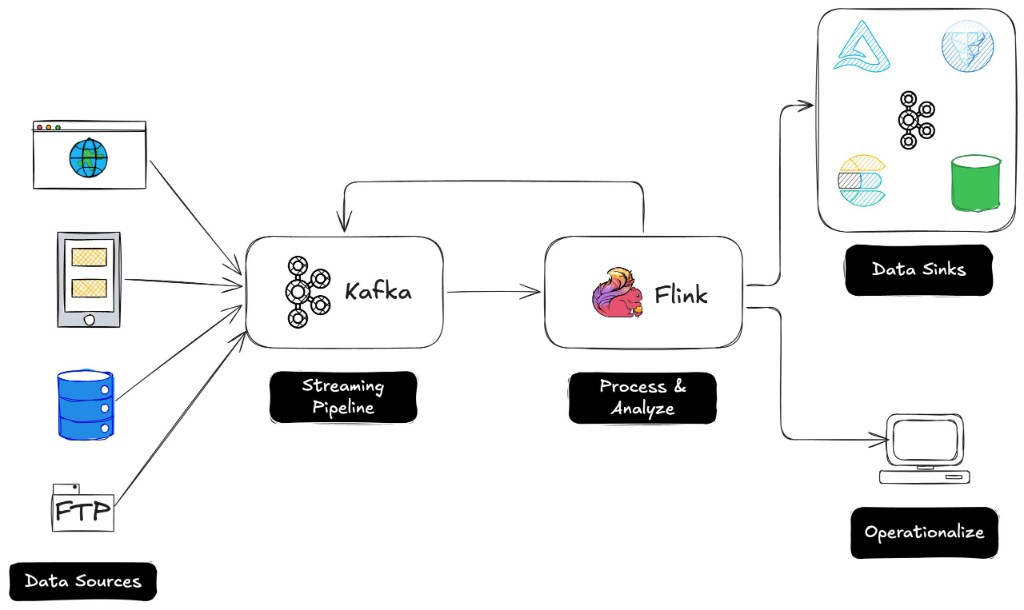
\includegraphics[width=\linewidth]{kafka_flink_pipeline.png}
    \end{column}
    \begin{column}{0.46\textwidth}
      \begin{itemize}
        \item Flink 作业通常承担持续运行的计算与写出职责。
        \item Kafka Topic 会随租户、日期、地域、灰度迁移、容灾切换而变化。
        \item 静态 KafkaSink 在作业构建阶段绑定目标 Topic，运行期缺少自动适配能力。
      \end{itemize}
      \begin{alertblock}{关注的问题}
        当可写 Topic 集合变化时，Sink 如何在不重启作业的前提下发现变化、更新写入路径，并保持状态与提交可恢复？
      \end{alertblock}
    \end{column}
  \end{columns}
\end{frame}

\begin{frame}{研究现状}
  \begin{table}
    \scriptsize
    \renewcommand{\arraystretch}{1.22}
    \gridtable
    \begin{tabularx}{\textwidth}{|L{0.18\textwidth}|L{0.28\textwidth}|Y|}
      \hline
      \rowcolor{cprimary!12}
      方案 & 已有能力 & 与目标需求的差异 \\
      \hline
      静态 KafkaSink & 固定 Topic 写入、写入一致性、事务提交 &
      目标在构建阶段绑定，缺少运行期正则发现和逻辑路由表。 \\
      \hline
      Source 正则订阅 & 消费端动态发现 Topic 与分区 &
      面向消费进度与分区管理，不能直接解决生产者、写入器、提交问题。 \\
      \hline
      Kafka Connect / 数据变更捕获 & 外部系统接入、任务级配置管理 &
      关注数据进入 Kafka/Flink，不负责 Flink Sink 内部多目标写出。 \\
      \hline
    \end{tabularx}
    \finishgridtable
  \end{table}
  \begin{alertblock}{现有工作不足}
    现有方案分别覆盖静态写入、Source 侧正则订阅和外部数据接入，但缺少面向 Flink Sink 侧的运行期 Topic 发现、动态路由、写入状态与提交恢复的一体化机制。
  \end{alertblock}
\end{frame}

\begin{frame}{问题建模与研究路线}
  \begin{center}
    \begin{tikzpicture}[
      node distance=0.95cm and 0.95cm,
      box/.style={draw, rounded corners, align=center, minimum width=2.35cm, minimum height=0.82cm, font=\small},
      arr/.style={-Stealth, thick}
    ]
      \node[box, fill=black!3] (meta) {Kafka 元数据\\Topic 集合};
      \node[box, fill=black!3, right=of meta] (pattern) {正则发现\\匹配 Topic};
      \node[box, fill=black!3, right=of pattern] (route) {逻辑路由\\映射物理 Topic};
      \node[box, fill=black!3, below=of route] (writer) {路由级写入器\\复用 KafkaSink};
      \node[box, fill=black!3, left=of writer] (state) {Checkpoint 状态\\与提交恢复};
      \draw[arr] (meta) -- (pattern);
      \draw[arr] (pattern) -- (route);
      \draw[arr] (route) -- (writer);
      \draw[arr] (writer) -- (state);
    \end{tikzpicture}
  \end{center}
  \begin{itemize}
    \item Topic 发现解决“有哪些目标可以写”。
    \item 逻辑路由解决“业务记录应写到哪类目标”。
    \item 路由级状态与提交解决“如何恢复和提交”。
  \end{itemize}
\end{frame}

\section{需求分析与系统设计}

\sectiondivider{第二部分}{需求分析与系统设计}{从运行期需求推导系统结构与关键流程}

\begin{frame}{功能需求分析}
  \tiny
  \begin{table}
    \renewcommand{\arraystretch}{1.12}
    \gridtable
    \begin{tabularx}{\textwidth}{|L{0.18\textwidth}|L{0.23\textwidth}|Y|L{0.24\textwidth}|}
      \hline
      \rowcolor{cprimary!12}
      需求类型 & 需求 & 产生原因 & 对系统的要求 \\
      \hline
      动态发现 & 运行期发现新增 Topic &
      业务流可能按日期、租户或数据类型持续产生新的写入目标。 &
      不重启作业即可感知目标变化，并把新目标纳入写入范围。 \\
      \hline
      路由解耦 & 业务路由与物理 Topic 解耦 &
      上游更适合表达业务含义，物理 Topic 名称会随部署和扩容变化。 &
      数据只携带稳定的业务路由，由 Sink 侧完成目标解析。 \\
      \hline
      状态恢复 & 动态目标下保持可恢复 &
      新增目标、已有目标和失败恢复后的目标都需要一致处理。 &
      路由关系、写入状态和待提交信息需要进入 Checkpoint。 \\
      \hline
      写入一致性 & 支持不同写入一致性要求 &
      实际场景既有低开销写入，也有 exactly-once 语义写入需求。 &
      动态能力不能绕开 KafkaSink 原有 Checkpoint 与提交机制。 \\
      \hline
    \end{tabularx}
    \finishgridtable
  \end{table}
  \begin{alertblock}{问题定义}
    静态 Sink 假设写入目标在作业启动前确定，而当前场景要求目标在运行期变化后仍能被发现、路由、写入和恢复。
  \end{alertblock}
\end{frame}

\begin{frame}{非功能指标}
  \scriptsize
  \begin{table}
    \renewcommand{\arraystretch}{1.18}
    \gridtable
    \begin{tabularx}{\textwidth}{|L{0.22\textwidth}|C{0.24\textwidth}|Y|}
      \hline
      \rowcolor{cprimary!12}
      指标类型 & 量化目标 & 取值依据 \\
      \hline
      发现实时性 & 首次写入延迟 $\leq 3$ s &
      元数据刷新周期为 2000 ms，并预留查询、调度和写入实例创建时间。 \\
      \hline
      吞吐可接受性 & 动态 2 路由下降 $\leq 5\%$ &
      动态层主要增加路由查找和写入实例管理，小规模场景下不应成为主导瓶颈。 \\
      \hline
      小规模扩展性 & 2 路由增至 4 路由下降 $\leq 10\%$ &
      用于判断 route 数翻倍后管理开销是否已明显压过输入侧限速。 \\
      \hline
      Checkpoint 协同 & 稳态完成时延 $\leq 100$ ms &
      Checkpoint 间隔为 5000 ms，稳态快照不应明显阻塞本地小规模 Job。 \\
      \hline
      exactly-once 语义 & 至少 5 次 Checkpoint 且双 Topic 有 committed 输出 &
      验证事务提交链路可运行，不外推为复杂故障注入下的完整证明。 \\
      \hline
    \end{tabularx}
    \finishgridtable
  \end{table}
  \begin{alertblock}{实验边界}
    本地 Kafka、单并行度、小规模路由和短时间运行窗口；指标用于原型验证。
  \end{alertblock}
\end{frame}

\begin{frame}{需求到设计的对应关系}
  \scriptsize
  \begin{table}
    \renewcommand{\arraystretch}{1.25}
    \gridtable
    \begin{tabularx}{\textwidth}{|L{0.18\textwidth}|L{0.24\textwidth}|L{0.30\textwidth}|Y|}
      \hline
      \rowcolor{cprimary!12}
      需求 & 设计决策 & 设计内容 & 预期效果 \\
      \hline
      动态发现 & 周期性元数据发现 &
      定时查询 Kafka Topic 集合，按命名规则筛选候选目标。 &
      新增 Topic 可在下一个发现周期进入系统。 \\
      \hline
      路由解耦 & 逻辑路由表 &
      用业务路由标识映射物理写入目标，数据事件不直接绑定 Topic。 &
      上游业务表达稳定，物理目标可独立调整。 \\
      \hline
      状态恢复 & 路由级状态组织 &
      以路由为粒度保存目标、写入状态和待提交信息。 &
      故障恢复时能重建对应目标的写入上下文。 \\
      \hline
      写入一致性 & 复用 KafkaSink Checkpoint 与提交路径 &
      动态层只管理目标变化，实际写出、状态快照和提交仍交给成熟机制。 &
      降低重复实现事务与提交逻辑的风险。 \\
      \hline
    \end{tabularx}
    \finishgridtable
  \end{table}
  \begin{alertblock}{总体原则}
    不是为每个 Topic 启动一套独立作业，而是在一个 Sink 内把“目标变化”转换为可管理的路由状态。
  \end{alertblock}
\end{frame}

\begin{frame}{总体设计：围绕需求组织的动态 Sink}
  \scriptsize
  \begin{columns}[T,onlytextwidth]
    \begin{column}{0.54\textwidth}
      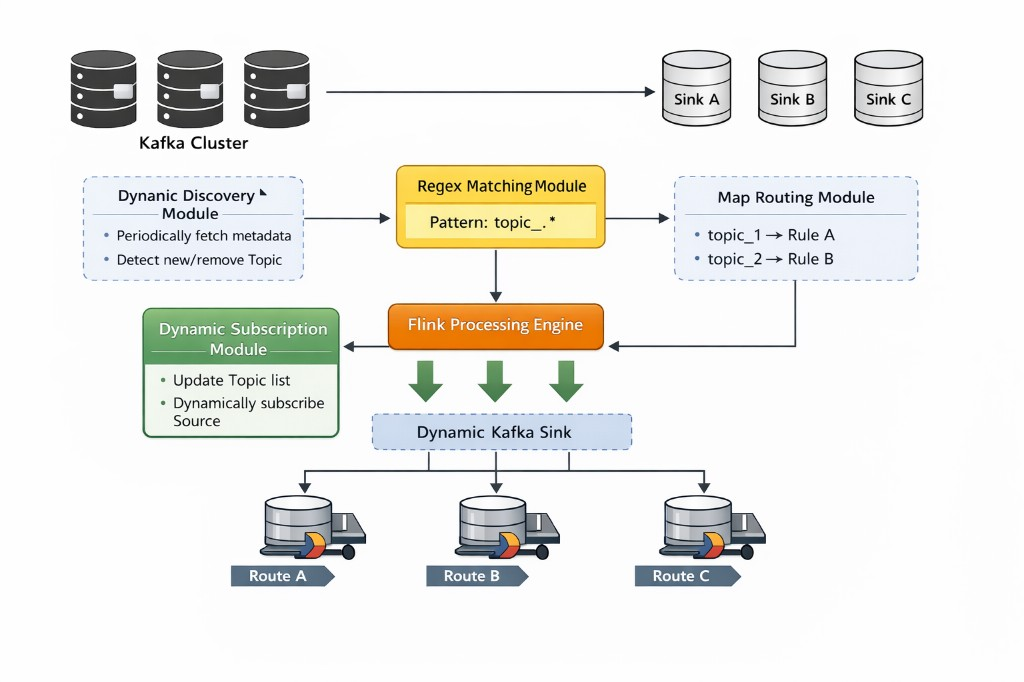
\includegraphics[width=\linewidth]{dynamic_sink_architecture.png}
    \end{column}
    \begin{column}{0.43\textwidth}
      \begin{table}
        \renewcommand{\arraystretch}{1.18}
        \gridtable
        \begin{tabularx}{\linewidth}{|L{0.32\linewidth}|Y|}
          \hline
          \rowcolor{cprimary!12}
          需求 & 架构响应 \\
          \hline
          动态发现 & 元数据发现层识别新增 Topic。 \\
          \hline
          路由解耦 & 运行时路由层解析业务路由。 \\
          \hline
          状态恢复 & 状态提交层保存路由级上下文。 \\
          \hline
          写入一致性 & 状态快照与提交复用 KafkaSink 能力。 \\
          \hline
        \end{tabularx}
        \finishgridtable
      \end{table}
      \vspace{0.15em}
      {\small\textbf{总体原则：}动态层只处理“目标会变”这一新增问题，避免重新实现底层生产者、事务和提交逻辑。}
    \end{column}
  \end{columns}
\end{frame}

\begin{frame}{动态发现：运行期发现新增 Topic}
  \small
  \begin{center}
    \begin{tikzpicture}[
      node distance=0.82cm and 0.9cm,
      box/.style={draw, rounded corners, align=center, font=\scriptsize, minimum width=2.35cm, minimum height=0.72cm},
      arr/.style={-Stealth, thick}
    ]
      \node[box, fill=black!3] (meta) {Kafka 元数据\\Topic 集合};
      \node[box, fill=black!3, right=of meta] (filter) {命名规则匹配\\候选目标};
      \node[box, fill=black!3, right=of filter] (diff) {目标集合对比\\新增 / 已有 / 移除};
      \node[box, fill=black!3, below=of diff] (active) {活跃目标集合\\可写 Topic};
      \node[box, fill=black!3, left=of active] (writer) {写入通道\\创建或复用};
      \draw[arr] (meta) -- (filter);
      \draw[arr] (filter) -- (diff);
      \draw[arr] (diff) -- (active);
      \draw[arr] (active) -- (writer);
    \end{tikzpicture}
  \end{center}
  \begin{table}
    \scriptsize
    \renewcommand{\arraystretch}{1.18}
    \gridtable
    \begin{tabularx}{\textwidth}{|L{0.24\textwidth}|Y|Y|}
      \hline
      \rowcolor{cprimary!12}
      设计点 & 解决的问题 & 边界控制 \\
      \hline
      周期性发现 & 避免新增 Topic 依赖作业重启。 & 发现周期设置为 2000 ms，实验按 3 s 首次写入目标验证。 \\
      \hline
      集合差分 & 区分新增目标和已有目标。 & 已有写入通道复用，新增目标才创建上下文。 \\
      \hline
    \end{tabularx}
    \finishgridtable
  \end{table}
\end{frame}

\begin{frame}{路由解耦：业务路由与物理 Topic 解耦}
  \small
  \begin{center}
    \begin{tikzpicture}[
      node distance=0.9cm and 0.95cm,
      box/.style={draw, rounded corners, align=center, font=\scriptsize, minimum width=2.35cm, minimum height=0.72cm},
      arr/.style={-Stealth, thick}
    ]
      \node[box, fill=black!3] (event) {数据事件\\业务路由标识};
      \node[box, fill=black!3, right=of event] (table) {路由表\\业务含义到目标};
      \node[box, fill=black!3, right=of table] (target) {物理目标\\Kafka Topic};
      \node[box, fill=black!3, below=of table] (control) {控制事件\\更新映射关系};
      \node[box, fill=black!3, right=of target] (write) {写入\\目标 Topic};
      \draw[arr] (event) -- (table);
      \draw[arr] (control) -- (table);
      \draw[arr] (table) -- (target);
      \draw[arr] (target) -- (write);
    \end{tikzpicture}
  \end{center}
  \begin{columns}[T,onlytextwidth]
    \begin{column}{0.48\textwidth}
      \begin{block}{需求侧}
        上游数据只表达“属于哪类业务流”，不感知具体 Topic 名称、集群地址和写入实例。
      \end{block}
    \end{column}
    \begin{column}{0.48\textwidth}
      \begin{block}{设计侧}
        路由表在 Sink 侧维护，控制事件负责更新映射，数据事件按当前映射选择目标。
      \end{block}
    \end{column}
  \end{columns}
\end{frame}

\begin{frame}{状态恢复：动态目标下保持可恢复}
  \small
  \begin{center}
    \begin{tikzpicture}[
      node distance=1.05cm and 1.2cm,
      state/.style={draw, rounded corners, align=center, minimum width=2.25cm, minimum height=0.72cm, font=\scriptsize},
      arr/.style={-Stealth, thick}
    ]
      \node[state, fill=black!3] (missing) {未发现\\Topic 不存在或不匹配};
      \node[state, fill=black!3, right=of missing] (resolved) {已解析\\生成物理写入目标};
      \node[state, fill=black!3, right=of resolved] (active) {活跃\\可接收数据写入};
      \node[state, fill=black!3, below=of active] (retired) {退役\\停止接收新数据};
      \node[state, fill=black!3, left=of retired] (restored) {恢复\\从 Checkpoint 重建};
      \draw[arr] (missing) -- node[above, font=\tiny]{发现 Topic} (resolved);
      \draw[arr] (resolved) -- node[above, font=\tiny]{创建写入实例} (active);
      \draw[arr] (active) -- node[right, font=\tiny]{Topic 消失或配置变更} (retired);
      \draw[arr] (restored) -- node[below, font=\tiny]{恢复后继续写入} (active);
      \draw[arr] (active) to[bend left=18] node[below, font=\tiny]{Checkpoint 保存} (restored);
    \end{tikzpicture}
  \end{center}
  \begin{alertblock}{设计要点}
    路由生命周期与 Checkpoint 绑定，新增目标不是临时变量，而是可恢复的运行时状态。
  \end{alertblock}
\end{frame}

\begin{frame}{写入一致性：Checkpoint 与提交机制}
  \small
  \begin{center}
    \begin{tikzpicture}[
      node distance=0.9cm and 0.95cm,
      box/.style={draw, rounded corners, align=center, font=\scriptsize, minimum width=2.25cm, minimum height=0.72cm},
      arr/.style={-Stealth, thick}
    ]
      \node[box, fill=black!3] (dynamic) {动态层\\发现与路由};
      \node[box, fill=black!3, right=of dynamic] (writer) {写入层\\KafkaSink};
      \node[box, fill=black!3, right=of writer] (topic) {Kafka Topic};
      \node[box, fill=black!3, below=of writer] (ckpt) {Checkpoint\\状态快照};
      \node[box, fill=black!3, right=of ckpt] (commit) {提交\\事务完成};
      \draw[arr] (dynamic) -- (writer);
      \draw[arr] (writer) -- (topic);
      \draw[arr] (writer) -- (ckpt);
      \draw[arr] (ckpt) -- (commit);
      \draw[arr] (commit) -- (topic);
    \end{tikzpicture}
  \end{center}
  \begin{table}
    \scriptsize
    \renewcommand{\arraystretch}{1.18}
    \gridtable
    \begin{tabularx}{\textwidth}{|L{0.25\textwidth}|Y|Y|}
      \hline
      \rowcolor{cprimary!12}
      写入要求 & 动态层职责 & 复用能力 \\
      \hline
      at-least-once 语义 & 选择目标、维护活跃写入上下文。 & 常规写入与 Checkpoint 快照。 \\
      \hline
      exactly-once 语义 & 按路由保存待提交信息，恢复后重建提交上下文。 & KafkaSink 原有 Checkpoint 与事务提交路径。 \\
      \hline
    \end{tabularx}
    \finishgridtable
  \end{table}
\end{frame}

\begin{frame}{小结：需求牵引下的设计闭环}
  \scriptsize
  \begin{table}
    \renewcommand{\arraystretch}{1.28}
    \gridtable
    \begin{tabularx}{\textwidth}{|L{0.18\textwidth}|L{0.27\textwidth}|L{0.28\textwidth}|Y|}
      \hline
      \rowcolor{cprimary!12}
      需求 & 关键设计 & 验证指标 & 验证目标 \\
      \hline
      动态发现 & 周期发现与目标集合差分 & 首次写入延迟 & 能否真正做到运行期扩写。 \\
      \hline
      路由解耦 & 逻辑路由表与控制事件 & 显式路由分布 & 能否把业务语义和 Topic 名称解耦。 \\
      \hline
      状态恢复 & 路由级状态与 Checkpoint 绑定 & Checkpoint 完成时延 & 动态目标是否还能恢复。 \\
      \hline
      写入一致性 & 复用 KafkaSink Checkpoint 与提交 & at-least-once 语义、exactly-once 语义运行结果 & 动态能力是否影响写入一致性。 \\
      \hline
    \end{tabularx}
    \finishgridtable
  \end{table}
  \begin{alertblock}{验证思路}
    后续实验围绕发现延迟、路由分布、Checkpoint 时延和写入一致性展开。
  \end{alertblock}
\end{frame}

\section{实验设计与结果分析}

\sectiondivider{第三部分}{实验设计与结果分析}{验证动态发现、吞吐开销、Checkpoint 和 exactly-once 语义}

\begin{frame}{实验设计：需求、Job 与指标一一对应}
  \scriptsize
  \begin{table}
    \renewcommand{\arraystretch}{1.18}
    \gridtable
    \begin{tabularx}{\textwidth}{|C{0.15\textwidth}|L{0.23\textwidth}|L{0.30\textwidth}|Y|}
      \hline
      \rowcolor{cprimary!12}
      验证目标 & 实验 Job & 观测指标 & 判定方式 \\
      \hline
      动态发现 & 自动发现 Job &
      Topic 创建到首次写入的延迟。 &
      最大延迟不超过 3 s。 \\
      \hline
      路由解耦 & 动态路由 Job &
      两个逻辑路由对应 Topic 的输出分布。 &
      输出能够按路由进入指定 Topic。 \\
      \hline
      吞吐可接受性 & 静态基线 Job + 动态 2 路由 Job &
      静态基线与动态写入吞吐。 &
      动态方案下降不超过 5\%。 \\
      \hline
      小规模扩展性 & 动态 2 路由 Job + 动态 4 路由 Job &
      路由数增加后的吞吐变化。 &
      2 到 4 路由下降不超过 10\%。 \\
      \hline
      写入一致性 & 容错提交 Job &
      Checkpoint 次数、事务输出、双 Topic 分布。 &
      至少 5 次 Checkpoint，且两个 Topic 有 committed 输出。 \\
      \hline
    \end{tabularx}
    \finishgridtable
  \end{table}
  \begin{alertblock}{实验条件}
    本地 Kafka、单并行度、小规模路由、短时间运行窗口。
  \end{alertblock}
\end{frame}

\begin{frame}{动态 Topic 发现验证}
  \scriptsize
  \begin{alertblock}{验证目标：动态发现}
    Topic 在运行期创建后，Sink 能够在不重启 Job 的情况下发现新增目标并开始写入。
  \end{alertblock}
  \begin{columns}[T,onlytextwidth]
    \begin{column}{0.34\textwidth}
      \metric{样本数}{6}
      \metric{平均延迟}{1.530 s}
      \metric{最大延迟}{2.418 s}
    \end{column}
    \begin{column}{0.62\textwidth}
      \begin{table}
        \tiny
        \renewcommand{\arraystretch}{1.03}
        \gridtable
    \begin{tabularx}{\linewidth}{|C{0.18\linewidth}|C{0.16\linewidth}|C{0.34\linewidth}|C{0.20\linewidth}|}
          \hline
          \rowcolor{cprimary!12}
          轮次 & Topic 编号 & 首次写入延迟 / s & 首次观测位置 \\
          \hline
          第 1 轮 & 1 & 1.077 & 14 \\
          \hline
          第 1 轮 & 2 & 2.412 & 23 \\
          \hline
          第 1 轮 & 3 & 1.095 & 8 \\
          \hline
          第 2 轮 & 1 & 1.103 & 14 \\
          \hline
          第 2 轮 & 2 & 2.418 & 24 \\
          \hline
          第 2 轮 & 3 & 1.074 & 10 \\
          \hline
        \end{tabularx}
        \finishgridtable
      \end{table}
      \begin{itemize}
        \item 2 s 轮询决定主要等待时间，实测还包含元数据查询、写入通道创建和消费端观测开销。
        \item 结果落在 1.074--2.418 s，最大值低于 3 s 阈值，验证自动发现路径可用。
      \end{itemize}
    \end{column}
  \end{columns}
\end{frame}

\begin{frame}{路由解耦验证}
  \scriptsize
  \begin{alertblock}{验证目标：路由解耦}
    输入数据携带逻辑路由标识，Sink 根据运行时路由映射选择物理 Topic，避免业务侧直接绑定 Topic 名称。
  \end{alertblock}
  \begin{columns}[T,onlytextwidth]
    \begin{column}{0.38\textwidth}
      \metric{Topic A 输出}{2812}
      \metric{Topic B 输出}{2930}
    \end{column}
    \begin{column}{0.58\textwidth}
      \begin{table}
        \tiny
        \renewcommand{\arraystretch}{1.06}
        \gridtable
        \begin{tabularx}{\linewidth}{|L{0.34\linewidth}|C{0.16\linewidth}|C{0.22\linewidth}|C{0.18\linewidth}|}
          \hline
          \rowcolor{cprimary!12}
          实验 Job & 目标数 & 输出总条数 & 输出占比 \\
          \hline
          动态 2 路由 Job & 2 & 5742 & 49.0\% / 51.0\% \\
          \hline
        \end{tabularx}
        \finishgridtable
      \end{table}
      \begin{itemize}
        \item 两个逻辑路由分别写入对应 Topic，输出均能被消费端观测。
        \item 输出分布接近输入侧轮转策略，说明运行时路由映射能够稳定控制写入目标。
      \end{itemize}
    \end{column}
  \end{columns}
\end{frame}

\begin{frame}{吞吐可接受性验证}
  \scriptsize
  \begin{alertblock}{验证目标：吞吐可接受性}
    在相同输入限速下，比较动态 2 路由 Job 与静态基线 Job 的吞吐差异。
  \end{alertblock}
  \begin{table}
    \tiny
    \renewcommand{\arraystretch}{1.05}
    \gridtable
    \begin{tabularx}{\textwidth}{|L{0.27\textwidth}|C{0.22\textwidth}|C{0.12\textwidth}|C{0.18\textwidth}|C{0.13\textwidth}|}
      \hline
      \rowcolor{cprimary!12}
      实验 Job & 语义 & 路由数 & 输出总条数 & 近似吞吐 \\
      \hline
      静态基线 Job & at-least-once 语义 & 1 & 5776 & 192.5 条/s \\
      \hline
      动态 2 路由 Job & at-least-once 语义 & 2 & 5742 & 191.4 条/s \\
      \hline
    \end{tabularx}
    \finishgridtable
  \end{table}
  \vspace{-0.2em}
  \begin{columns}[T,onlytextwidth]
    \begin{column}{0.48\textwidth}
      \begin{block}{输入限速}
        \begin{align*}
          \text{recordsPerSecond} &= 1000 / \text{emitIntervalMs} \\
                                  &= 1000 / 5 \approx 200
        \end{align*}
      \end{block}
    \end{column}
    \begin{column}{0.48\textwidth}
      \begin{itemize}
        \item 动态 2 路由相比静态基线吞吐下降约 0.59\%，低于 5\% 阈值。
        \item 当前 191--193 条/s 接近输入侧 200 条/s 上限。
        \item 这里比较的是动态 Sink 额外开销，不是 Kafka/Flink 峰值压测。
      \end{itemize}
    \end{column}
  \end{columns}
\end{frame}

\begin{frame}{小规模扩展性验证}
  \scriptsize
  \begin{alertblock}{验证目标：小规模扩展性}
    路由数从 2 增加到 4 后，观察动态写入吞吐是否出现明显退化。
  \end{alertblock}
  \begin{table}
    \tiny
    \renewcommand{\arraystretch}{1.05}
    \gridtable
    \begin{tabularx}{\textwidth}{|L{0.28\textwidth}|C{0.20\textwidth}|C{0.16\textwidth}|C{0.16\textwidth}|C{0.14\textwidth}|}
      \hline
      \rowcolor{cprimary!12}
      实验 Job & 语义 & 输出总条数 & 近似吞吐 & 相对变化 \\
      \hline
      动态 2 路由 Job & at-least-once 语义 & 5742 & 191.4 条/s & 基准 \\
      \hline
      动态 4 路由 Job & at-least-once 语义 & 5763 & 192.1 条/s & 上升约 0.37\% \\
      \hline
    \end{tabularx}
    \finishgridtable
  \end{table}
  \begin{itemize}
    \item 2 路由到 4 路由没有出现超过 10\% 的吞吐下降。
    \item 在本地单并行度、小规模路由条件下，路由表查找和写入实例管理没有形成主要瓶颈。
    \item 更高并行度、更多路由和长时间运行仍需要进一步压力测试。
  \end{itemize}
\end{frame}

\begin{frame}{Checkpoint 协同与事务路径可运行性验证}
  \scriptsize
  \begin{alertblock}{验证目标：写入一致性}
    动态目标变化不能破坏 Checkpoint 协同和 exactly-once 语义下的事务提交路径。
  \end{alertblock}
  \begin{columns}[T,onlytextwidth]
    \begin{column}{0.48\textwidth}
      \begin{block}{Checkpoint 协同}
        \begin{itemize}
          \item 约 22 秒内观察到连续 5 次成功 Checkpoint。
          \item 完成时延：476 ms、11 ms、22 ms、19 ms、21 ms。
          \item 去除首次冷启动后，稳态平均约 18.2 ms。
        \end{itemize}
      \end{block}
    \end{column}
    \begin{column}{0.48\textwidth}
      \begin{block}{exactly-once 语义可运行性}
        \begin{itemize}
          \item 成功完成 5 次 Checkpoint。
          \item 输出总条数 2092，近似吞吐 95.1 条/s。
          \item 两个目标 Topic 输出为 1084 / 1008。
        \end{itemize}
      \end{block}
    \end{column}
  \end{columns}
  \begin{alertblock}{验证范围}
    该实验验证小规模事务路径可运行，但不等同于复杂故障注入下的完整端到端 exactly-once 语义证明。
  \end{alertblock}
\end{frame}

\begin{frame}{对比实验与方案优势分析}
  \scriptsize
  \begin{columns}[T,onlytextwidth]
    \begin{column}{0.38\textwidth}
      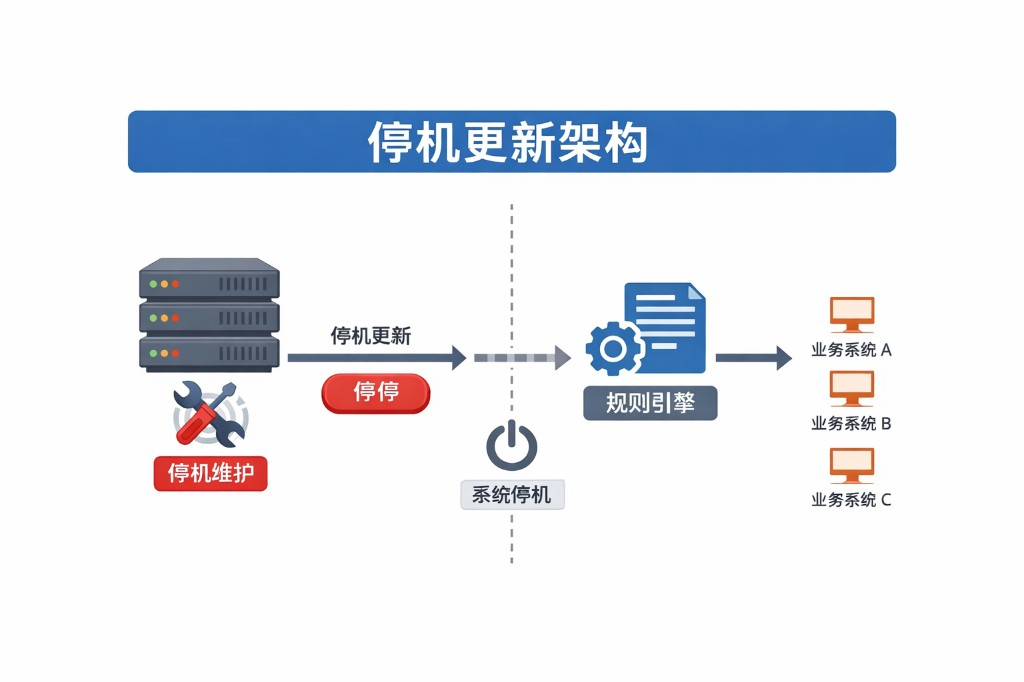
\includegraphics[width=\linewidth]{offline_update_architecture.png}
    \end{column}
    \begin{column}{0.58\textwidth}
      \begin{block}{静态 KafkaSink}
        构建阶段固定 Topic；实现简单，但目标变化时通常需要停机改配置。
      \end{block}
      \begin{block}{动态 Sink}
        运行期发现 Topic 并维护路由映射；路由级保存状态和提交信息。
      \end{block}
      \begin{alertblock}{主要成本}
        引入元数据轮询、多写入实例管理和提交包装。
      \end{alertblock}
    \end{column}
  \end{columns}
  \vspace{0.3em}
  Topic 集合长期稳定时静态 KafkaSink 更简单；Topic 频繁增删或迁移时动态 Sink 更有价值。
\end{frame}

\section{总结与展望}

\sectiondivider{第四部分}{总结与展望}{归纳工作贡献，并说明当前边界和后续方向}

\begin{frame}{研究工作总结}
  \begin{columns}[T,onlytextwidth]
    \begin{column}{0.32\textwidth}
      \begin{block}{Sink 侧动态发现}
        Kafka 元数据轮询 + 正则匹配，新增 Topic 最大 2.418 s 内开始写入。
      \end{block}
    \end{column}
    \begin{column}{0.32\textwidth}
      \begin{block}{逻辑路由解耦}
        业务路由标识与物理 Topic 分离，支持运行期路由配置更新。
      \end{block}
    \end{column}
    \begin{column}{0.32\textwidth}
      \begin{block}{路由级容错提交}
        路由状态与提交信息纳入 Checkpoint 和提交器。
      \end{block}
    \end{column}
  \end{columns}
  \begin{itemize}
    \item 动态 2 路由相对静态基线吞吐下降约 0.59\%。
    \item 稳态 Checkpoint 时延约 18.2 ms。
    \item exactly-once 语义小规模运行完成 5 次 Checkpoint 且双 Topic 输出。
  \end{itemize}
\end{frame}

\begin{frame}{存在的不足与未来工作展望}
  \begin{enumerate}
    \item 元数据访问优化：当前依赖周期性全量查询，后续可引入缓存、增量发现和多集群元数据服务。
    \item 资源生命周期：路由数增长会带来写入器和生产者资源压力；exactly-once 语义下退役写入器安全回收仍需完善。
    \item 一致性验证：需要故障注入、任务恢复、事务超时、可提交读消费校验等端到端测试。
    \item 性能评估：扩展到更高并行度、更多路由、更长运行时间和真实数据流。
  \end{enumerate}
  \begin{alertblock}{适用范围}
    当前验证表明，本地单机、小规模路由场景下动态 Kafka Sink 机制可行；生产级服务保障和复杂故障场景属于后续工程化工作。
  \end{alertblock}
\end{frame}

\makebottom

\end{document}
